% !TeX root = Report.tex
\documentclass[conference]{IEEEtran}
\bibliographystyle{IEEEtran}

\usepackage[none]{hyphenat}

\usepackage{color}
\usepackage{graphicx}
\usepackage{caption}
\usepackage{flafter}
\usepackage{placeins}
\usepackage{cite}
\usepackage{float}
%-------------------------------------------------------------------------------

\newcommand{\micro}{\textmu}
\newcommand{\Ohm}{$\Omega$}
\newcommand{\MATLAB}{\textsc{Matlab}\xspace}

\newcommand{\etal}       {\emph{et~al.}}
\newcommand{\ie}         {i.e.}
\newcommand{\bookcite}[2]{\cite{#1}~pg.~#2}
%-------------------------------------------------------------------------------

\newcounter{author}
\renewcommand{\theauthor}{\stepcounter{author}\raisebox{1ex}{\small\fnsymbol{author}}}
%-------------------------------------------------------------------------------

\renewcommand{\today}{%
 \number\day\space%
 \ifcase\month%
  \or January%
  \or February%
  \or March%
  \or April%
  \or May%
  \or June%
  \or July%
  \or August%
  \or September%
  \or October%
  \or November%
  \or December%
 \fi%
 \space\number\year%
}
%-------------------------------------------------------------------------------

\newlength{\TempFigureLength}
%-------------------------------------------------------------------------------

\newenvironment{FigureEnvironment}{
 \begin{figure}[!t]%
 \begin{center}%
}{
 \end{center}%
 \end{figure}%
}
%-------------------------------------------------------------------------------

\def\FigureSize{0.8}

\newcommand{\Figure}[3][scale=\FigureSize]{%
 \begin{FigureEnvironment}%
  \refstepcounter{figure}
  \addcontentsline{lof}{section}{Fig.~\thefigure{}~~~#2}
  \label{fig:#3}%
  \includegraphics[#1]{Figures/#3}\\[1em]%
  \footnotesize
  \settowidth{\TempFigureLength}{Fig.~\thefigure{}.~~{#2}}
  \ifdim \TempFigureLength > 0.95\columnwidth
   \parbox{0.95\columnwidth}{Fig.~\thefigure{}.~~{#2}}%
  \else
   Fig.~\thefigure{}.~~{#2}%
  \fi
 \end{FigureEnvironment}%
}
%-------------------------------------------------------------------------------

\newenvironment{TableEnvironment}{
 \begin{table}[H]%
 \begin{center}%
}{
 \end{center}%
 \end{table}%
}
%-------------------------------------------------------------------------------

\renewcommand{\thetable}{\Roman{table}}

\newcommand{\Table}[5]{%
 \begin{TableEnvironment}%
  \refstepcounter{table}
  \addcontentsline{lot}{section}{TABLE \thetable{}~~~#1}
  \label{tab:#5}%
  TABLE \thetable{}\\[1ex]
  \settowidth{\TempFigureLength}{\textsc{#1}}
  \ifdim \TempFigureLength > 0.95\columnwidth
   \parbox{0.95\columnwidth}{\textsc{#1}}%
  \else
   \textsc{#1}%
  \fi\\[1em]
  \renewcommand{\arraystretch}{1.2}
  \begin{tabular}{#2}
   \hline
   \hline
    #3\\
   \hline
    #4
   \hline
   \hline
  \end{tabular}
 \end{TableEnvironment}%
}
%-------------------------------------------------------------------------------

\newcommand{\Plot}[2]{
 \begin{FigureEnvironment}%
  \refstepcounter{figure}
  \addcontentsline{lof}{section}{Fig.~\thefigure{}~~~#1}
  \label{fig:#2}%
  \includegraphics[width=0.95\columnwidth]{../../Octave/Prac_1/#2}\\[1em]%
  \footnotesize
  \settowidth{\TempFigureLength}{Fig.~\thefigure{}.~~{#1}}
  \ifdim \TempFigureLength > 0.95\columnwidth
   \parbox{0.95\columnwidth}{Fig.~\thefigure{}.~~{#1}}%
  \else
   Fig.~\thefigure{}.~~{#1}%
  \fi
 \end{FigureEnvironment}%
}
\usepackage{textcomp} %Used in listings for printing upright quotes
\usepackage{listings} %For typesetting source code
\lstloadlanguages{C++, Matlab, Verilog}
%-------------------------------------------------------------------------------

\lstset{%
 frame      = single,%
 basicstyle = \tiny\ttfamily,%
 basewidth  = 1.3ex%
% basicstyle = \scriptsize\ttfamily,%
% basewidth  = 1.2ex%
}
%-------------------------------------------------------------------------------

\definecolor{keyword}{rgb}{0.5, 0.0, 0.0}
\definecolor{comment}{rgb}{0.0, 0.5, 0.0}
\definecolor{string} {rgb}{0.0, 0.0, 0.7}
\definecolor{define} {rgb}{1.0, 0.5, 0.0}
\definecolor{string2}{rgb}{0.5, 0.0, 0.5}
%-------------------------------------------------------------------------------

\newcounter{Listing}
\renewcommand{\theListing}{\arabic{Listing}}

\newlength{\CodeWidth}

\newcommand{\StartListing}[2]{
 \setlength{\CodeWidth}{0.95\columnwidth}
 \figure[!t]
 \refstepcounter{Listing}
 \addcontentsline{lof}{section}{Listing \theListing{}~~~#1}
 \label{lst:#2}
 \def\ListingCaption{#1}
 \noindent\centering\minipage{\CodeWidth}%
}
\newcommand{\EndListing}{
 \endminipage\\%
 {%
  \footnotesize%
  \settowidth{\TempFigureLength}{Listing~\theListing{}.~~\ListingCaption}%
  \ifdim \TempFigureLength > 0.95\columnwidth%
   \parbox{0.95\columnwidth}{Listing~\theListing{}.~~\ListingCaption}%
  \else%
   Listing~\theListing{}.~~\ListingCaption%
  \fi%
 }%
 \endfigure%
}

\newcommand{\StartListingInline}{%
 \setlength{\CodeWidth}{0.95\columnwidth}%
 \noindent\centering\minipage{\CodeWidth}%
}
\newcommand{\EndListingInline}  {\endminipage\par}
%-------------------------------------------------------------------------------

\newcommand{\SetupMatlab}{
 \lstset{%
  language         = Matlab,%
  upquote          = true,%
  showstringspaces = false,%
  keywordstyle     = {\color{keyword}\slshape},%
  commentstyle     = {\color{comment}},%
  stringstyle      = {\color{string}},
  morecomment      = [l][\color{comment}]{\#}%
 }%
}

\lstnewenvironment{Matlab_float}[2]{
 \SetupMatlab
 \StartListing{#1}{#2}
}{
 \EndListing
}

\lstnewenvironment{Matlab}{
 \SetupMatlab
 \StartListingInline
}{
 \EndListingInline
}
%-------------------------------------------------------------------------------

\newcommand{\SetupGLSL}{
 \lstset{%
  language=C,%
  upquote=true,%
  showstringspaces=false,%
  keywordstyle=   {\color{keyword}\slshape},%
  commentstyle=   {\color{comment}},%
  stringstyle =   {\color{string}},%
  morecomment =[l][\color{define}]{\#},%
  morekeywords={%
   in,%
   out,%
   vec2,%
   vec3,%
   vec4,%
   sin,%
   length,%
   texture2D,%
   sampler2D,%
   gl_FragColor,%
   varying,%
   uniform,%
   discard%
  }%
 }%
}

\lstnewenvironment{GLSL_float}[2]{
 \SetupGLSL
 \StartListing{#1}{#2}
}{
 \EndListing
}

\lstnewenvironment{GLSL}{
 \SetupGLSL
 \StartListingInline
}{
 \EndListingInline
}
%-------------------------------------------------------------------------------

\newcommand{\SetupOpenCL}{
 \lstset{%
  language=C,%
  upquote=true,%
  showstringspaces=false,%
  keywordstyle=   {\color{keyword}\slshape},%
  commentstyle=   {\color{comment}},%
  stringstyle =   {\color{string}},%
  morecomment =[l][\color{define}]{\#},%
  morekeywords={%
   __kernel,%
   __global,%
   __local,%
  get_global_id%
  }%
 }%
}

\lstnewenvironment{OpenCL_float}[2]{
 \SetupOpenCL
 \StartListing{#1}{#2}
}{
 \EndListing
}

\lstnewenvironment{OpenCL}{
 \SetupOpenCL
 \StartListingInline
}{
 \EndListingInline
}
%-------------------------------------------------------------------------------

\newcommand{\SetupVerilog}{
 \lstset{%
  language=Verilog,%
  upquote=true,%
  showstringspaces=false,%
  keywordstyle=   {\color{keyword}\slshape},%
  commentstyle=   {\color{comment}},%
  stringstyle =   {\color{string}},%
  morecomment =[l][\color{define}]{`}%
 }%
}

\lstnewenvironment{Verilog_float}[2]{
 \SetupVerilog
 \StartListing{#1}{#2}
}{
 \EndListing
}

\lstnewenvironment{Verilog}{
 \SetupVerilog
 \StartListingInline
}{
 \EndListingInline
}
%-------------------------------------------------------------------------------

\newcommand{\SetupCpp}{
 \lstset{%
  language         = C++,%
  upquote          = true,%
  showstringspaces = false,%
  keywordstyle     = {\color{keyword}\slshape},%
  commentstyle     = {\color{comment}},%
  stringstyle      = {\color{string}}%
 }%
}

\lstnewenvironment{Cpp_float}[2]{
 \SetupCpp
 \StartListing{#1}{#2}
}{
 \EndListing
}

\lstnewenvironment{Cpp}{
 \SetupCpp
 \StartListingInline
}{
 \EndListingInline
}
%-------------------------------------------------------------------------------

\usepackage[pdftex                       ,%
            bookmarks         = true     ,%
            bookmarksnumbered = true     ,%
            setpagesize       = false    ,%
            colorlinks        = true     ,%
            linkcolor         = black    ,%
            urlcolor          = black    ,%
            citecolor         = black    ,%
            pdfpagelayout     = OneColumn,%
            pdfstartview      = FitH]{hyperref}
%-------------------------------------------------------------------------------

%-------------------------------------------------------------------------------


\title{Practical 2 – MATLAB Parallel Computing Toolkit}

\author{%
 \setcounter{author}{1}
 \IEEEauthorblockN{Cammaran Clark and Kian Frassek}
 \setcounter{author}{1}
 \IEEEauthorblockA{%
  EEE4021 Class of 20\\
  University of Cape Town\\
  South Africa\\
  \theauthor{}CLRCAM007~~\theauthor{}FRSKIA001\\
 }
}

\begin{document}
\begin{sloppypar}

\maketitle

% We're using separate files for each main section
% Please see the subdirectories Body/.. for the files.

\begin{abstract}
\end{abstract}


\section{Introduction}
A Field Programmable Gate Array (FPGA) is an interconnected circuit which can be coding using Verilog and can be customized for specific applications.
This project details the building of a simple Trigger Surround Cache (TSC) using an ADC and a ring buffer memory device; an ADC records an input analog signal and converts it to a digital signal.
A ring buffer is a type of storage method where you have a fixed size storage, and you have two pointers: a read pointer which is also called the head and a write pointer which is also called the tail.
The TSC will also be able to communication with other devices using a clocked serial data transfer protocol.

\section{Methodology}

\subsection{Hardware}
The hardware used to conduct these experiments is a MacBook Pro 13" 2019 model.
All of these parallel programs were conducted on the GPU which is a Intel Iris Plus Graphics 1536 MB.
All of the single thread programs were conducted on the CPU which is 2 GHz Quad-Core Intel Core i5.

\subsection{Implementation}

\subsubsection{Single Thread Program}
The single thread program is a relative simple implementation in C code.
It requires two for loops which iterate over the row and column of the result matrix and a third which calculates the dot product of the input matrices to find the value of the cell of the output matrix.
There is one additional for loop which allows for multiplying a given number of matrices together

\begin{OpenCL}{C++ code to perform single threaded matrix multiplication}{C_Matrix_Mult}
 int matrix_output[matrix_size], matrixA[matrix_size], cell;
 for (int c = 0; c < matrix_size; c++) matrixA[c] = matrices[0][c];

 //Matrix multiplication
 for (int m = 1; m < MATRIX_COUNT; m++) {
  for (int row = 0; row < Size; row++) {
   for (int col = 0; col < Size; col++) {
    cell = 0;
    for (int dot = 0; dot < Size; dot++) {
     cell += matrixA[row * Size + dot] * matrices[m][col + dot * Size];
    }
    matrix_output[row * Size + col] = cell;
   }
  }
  //rewrite matrix A with output so loop can re-iterate
  for (int c = 0; c < matrix_size; c++) matrixA[c] = matrix_output[c];
 }
\end{OpenCL}

\subsubsection{Parallel Program}
The parallel program involves setting up OpenCL to run instances of a kernel program.
The kernel program itself runs a very similar instance of the cell calculation for the single thread program above where the row is equivalent to the workGroupNumber and the column is equivalent to the localGroupID.
A for loop is used to calculate the dot product as in the single thread program.
Lastly, there is an additional for loop in the OpenCL setup code which allows for successive matrix multiplication.


\begin{OpenCL}{OpenCL kernel code to perform parallel threaded matrix multiplication}{OpenCL_Matrix_Mult}
 __kernel void matrixMultiplication(
  __global int* matrixA_buffer,
  __global int* matrixB_buffer,
  __global int* output_buffer
 ){
  int workItemNum = get_global_id(0); //Work item ID
  int workGroupNum = get_group_id(0); //Work group ID
  int localGroupID = get_local_id(0); //Work items ID within each work group
  int localSize = get_local_size(0); //Get the work number of items per group

  //Row <=> workGroupNum; Column <=> localGroupID
  //workItemNum <=> workGroup * localSize + localGroupID
  int cell = 0;
  for (int i = 0; i < localSize; i++) {
   cell = cell + *(matrixA_buffer + workGroupNum * localSize + i) *
    *(matrixB_buffer + localGroupID + i * localSize);
  }
  *(output_buffer + workItemNum) = cell;
 }
\end{OpenCL}

\subsubsection{Code Verification}
Both the single thread and parallel program will undergo tests to ensure their correct functionality before their performances are evaluated.
The two programs will carry out the following known matrix multiplication as well as a similar version with matrix sizes of 5:

\vspace{5pt}
\begin{bmatrix}
 1 & 2 & 3 \\
 1 & 2 & 3 \\
 1 & 2 & 3
\end{bmatrix}
\begin{bmatrix}
 2 & 4 & 6 \\
 2 & 4 & 6 \\
 2 & 4 & 6
\end{bmatrix}
\begin{bmatrix}
 1 & 2 & 3 \\
 1 & 2 & 3 \\
 1 & 2 & 3
\end{bmatrix}
=
\begin{bmatrix}
 72 & 144 & 216 \\
 72 & 144 & 216 \\
 72 & 144 & 216
\end{bmatrix}
\vspace{5pt}

\subsection{Experiment Procedure}

To evaluate the performance of the single thread versus parallel program two experiments will be conducted and evaluate the difference in time taken and the speed up of the parallel program.
The first will be multiplying two matrices with different sizes, and the second will be to multiply different numbers of successive matrices of the same size.
All matrices of any size will follow the following format for a matrix of size $n \times n$:

\vspace{5pt}
\begin{bmatrix}
 1 & 2 & \dots & n\\
 1 & 2 & \dots & n\\
 \vdots & \vdots & \ddots & \vdots\\
 1 & 2 & \dots & n\\
\end{bmatrix}
\vspace{5pt}

Importantly, both tests will take an average of several tests in order to maximise accuracy and the parallel program will be run additional times before starting its data collection to warm up the cache.
Both methods of testing have different amounts of parallelization and different amounts of overhead and should give good understanding of the effectiveness of parallelizing matrix multiplication code.
\section{Results of Part 2}

\subsection{Question A}
The bubble sort function was created based off of sudo code for a generalised bubble sort.
The code is shown below

\begin{Matlab}
 function array = BubbleSort(array)
  for i = 1:length(array)
   for j = length(array):-1:i+1
    if array(j) > array(j-1)
     temp = array(j);
     array(j) = array(j-1);
     array(j-1) = temp;
    end
   end
  end
 return;
 end
\end{Matlab}

This code took 0.0087 seconds to sort the 100x100 matrix

\subsection{Question B}
The code to test the user function is shown below.
'timetaken' is a matrix for storing the times of both the user and inbuilt functions.

\begin{Matlab}
 % Initialize array
 testsizes = [100; 200; 500; 1000; 10000];%grid sizes tested
 timetaken = cell(1+length(testsizes),4);
 timetaken(1,:) = {"size", "bubble sort time", "inbuilt sort time", "speed up"};
 timetaken(2:end,1) = num2cell(testsizes); 

 % Loop over each row in timetaken
 for i = 2:size(timetaken,1)
  % Call the timetest function 
  %with the value in the first column (grid size) of the i-th row
  [timeBubble, timeInbuilt] = timetest(timetaken{i,1});
  timetaken{i,2} = timeBubble;
  timetaken{i,3} = timeInbuilt;
  % Calculate speed up
  timetaken{i,4} = timeBubble/timeInbuilt;
 end
 disp(timetaken)
\end{Matlab}

The function 'timetest' is given below.
It takes a matrix size, creates a square matrix, and then outputs the sort time for both the user and inbuilt functions.



\begin{Matlab}
 function [t_user,t_inbulit ] = timetest(size)

  X=rand(size, size);
  Y=X;

  tic
  for i = 1:size
   X(:,i) = BubbleSort(X(:,i));
  end
  t_user = toc();

  tic
  for i = 1:size
   Y(:,i) = sort(Y(:,i));
  end
  t_inbulit = toc();

  display("Time tacken by the bubble sort function was " + t_user " s.")
  display(" s. Time tacken by the inbuilt sort function was: "+  t_inbulit +" s.")

  return;
 end
\end{Matlab}

The results from the tests are shown in the table below

\Table{User vs inbuilt sort function}{lrrr}{
 \textbf{Matrix size} & \textbf{User} & \textbf{Inbuilt} & \textbf{Speed up}
}{
 100 & 0.0087 & 0.0002 & 40.507 \\
 200 & 0.0205 & 0.0003 & 62.791 \\
 500 & 0.1780 & 0.0012 & 145.18 \\
 1000 & 2.1324 & 0.0048 & 445.16 \\
 1000 & 1813.9 & 1.5631 & 1160.4 \\
}{2btbl}

\begin{figure}[H]
 \centering
 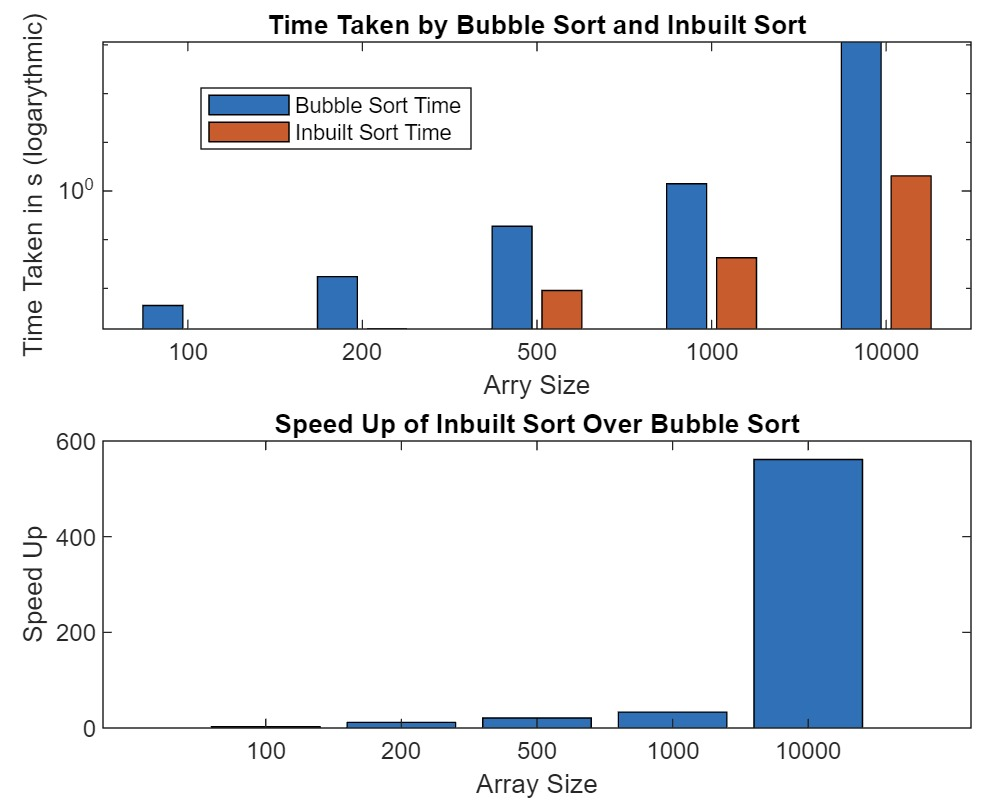
\includegraphics[width=0.6\columnwidth]{Figures/noPar}
 \caption{User vs inbuilt sort function}
 \label{fig:noPar}
\end{figure}

These results are logical because the inbuilt sort function uses the Quick Sort algorithm. 
This means that the bubble sort function has a big O notation of $O(n^2)$, while the inbuilt sort function has a big O notation of $O(n\log(n))$ in most cases.
This means that the inbuilt sort function will be faster than the bubble sort function for all sizes.
However, the time difference will be more pronounced as the size of the matrix increases.

Since the time taken by the BubbleSort algorithm increases at a faster rate than the inbuilt sort function, the speed up will increase as the size of the matrix increases.

\subsection{Question C}
The code to test the parallelism  user function is shown below.
'timetaken' is a matrix for storing the times of both the user and inbuilt functions.

\begin{Matlab}
 testsizes = [100, 5000];
 timetaken_par = cell(1+length(testsizes),4);
 timetaken_par(1,:) = {"size", "bubble sort time", "inbuilt sort time", "speed up"};
 timetaken_par(2:end,1) = num2cell(testsizes); 

 % Loop over each row in timetaken_par
 for i = 2:size(timetaken_par,1)
  % Call the timetest function with the value in the first column of the i-th row
  timeBubble = timebubble_parallelism(timetaken_par{i,1});
  timeInbuilt = timesort_parallelism(timetaken_par{i,1});
  timetaken_par{i,2} = timeBubble;
  timetaken_par{i,3} = timeInbuilt;
  % Calculate speed up
  timetaken_par{i,4} = timeBubble/timeInbuilt;
 end

 % Display the results
 disp(timetaken_par)
\end{Matlab}

The function 'timesort\_parallelism' simply returns the time to sort a square matrix of a given size using the inbuilt sort function.
The function 'timebubble\_parallelism' is given below.
It takes a matrix size, creates a square matrix, and then outputs the sort time for the user parallelism bubble-sort function.

\begin{Matlab}
function t_user = timebubble_parallelism(size)
    X=rand(size, size);
    tic
    spmd
        myStart = (spmdIndex - 1) * size/4 + 1;
        myEnd = myStart + size/4-1; 
        for i = myStart:myEnd
            X(:,i) = BubbleSort(X(:,i));
        end
    end
    t_user = toc();
    
    display("Time tacken by the parallelism bubble sort function was " + t_user );
    return;
end
\end{Matlab}

The results from the tests are shown in the table below

\Table{User vs inbuilt sort function}{lrrr}{
 \textbf{Matrix size} & \textbf{parallelized BubbleSort} & \textbf{Inbuilt} & \textbf{Speed up}
}{
 100 & 0.7642 & 0.001 & 764.96 \\
 5000 & 111.7174 & 1.0715 & 104.26 \\
}{2ctbl}

\begin{figure}[H]
 \centering
 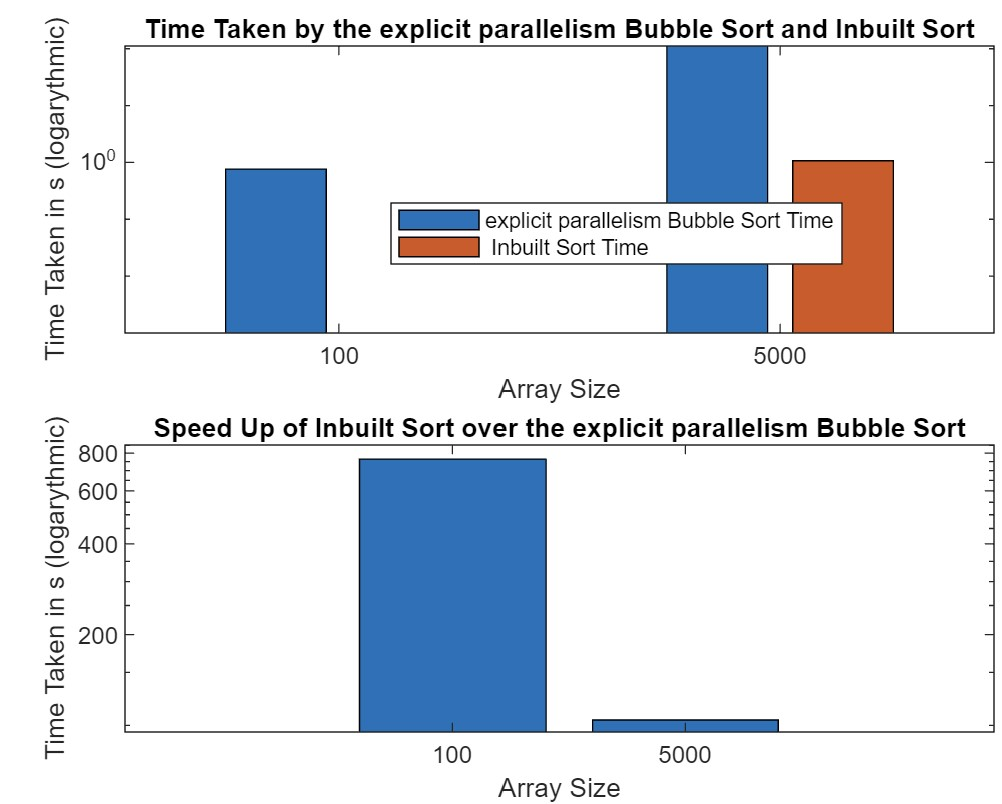
\includegraphics[width=0.6\columnwidth]{Figures/expPar_2}
 \caption{User parallelism vs inbuilt sort function}
 \label{fig:expPar}
\end{figure}

The results show that the sort function is faster than the parallelism bubble sort function.
This is because when the parallelize BubbleSort run on a nxn matrix the big O notation is $O(n×(n^2/p))$ where p is the number of workers in the parallel pool. 
The inbuilt sort function has a big O notation of $O(n×(n*log(n)))$.(There is an extra n because every column need to be sorted).

It makes sense for the speed up to slow down as the size of the matrix increases form 100 to 5000 as building the SPMD function takes time. this will hav a more noticeable effect lower-sized arrays.

\section{Conclusion}

The experiments show tha that small matrix sizes, single-threaded matrix multiplication is faster due to over heads.
As the matrix size increases, parallelized multiplication becomes quicker due to overhead becoming negligible relative to computation time.
The overhead includes OpenCL setup overheads and kernel startup overheads, with the former being constant and the latter increasing linearly with matrix count.
Due to the kernel startup overheads , parallelization efficiency improves slightly with larger matrix counts.
Overall, parallelized multiplication offers significant speedup for larger matrices compared to the single-threaded approach.

\bibliography{Bibliography/Bibliography}

\end{sloppypar}
\end{document}